% To je predloga za poročila o domačih nalogah pri predmetih, katerih
% nosilec je Tomaž Curk. Avtor predloge je Blaž Zupan.
%
% Seveda lahko tudi dodaš kakšen nov, zanimiv in uporaben element,
% ki ga v tej predlogi (še) ni. Več o LaTeX-u izveš na
% spletu, na primer na http://tobi.oetiker.ch/lshort/lshort.pdf.
%
% To predlogo lahko spremeniš v PDF dokument s pomočjo programa
% pdflatex, ki je del standardne instalacije LaTeX programov.

\documentclass[a4paper,11pt]{article}
\usepackage{a4wide}
\usepackage{fullpage}
\usepackage[utf8x]{inputenc}
\usepackage[slovene]{babel}
\selectlanguage{slovene}
\usepackage[toc,page]{appendix}
\usepackage[pdftex]{graphicx} % za slike
\usepackage{setspace}
\usepackage{color}
\definecolor{light-gray}{gray}{0.95}
\usepackage{listings} % za vključevanje kode
\usepackage{hyperref}
\renewcommand{\baselinestretch}{1.2} % za boljšo berljivost večji razmak
\renewcommand{\appendixpagename}{Priloge}


\lstset{% nastavitve za izpis kode, sem lahko tudi kaj dodaš/spremeniš
language=Python,
basicstyle=\footnotesize,
basicstyle=\ttfamily\footnotesize\setstretch{1},
backgroundcolor=\color{light-gray},
}

\title{6. Domača naloga}
\author{Marko Grešak (63130058)}
\date{\today}

\begin{document}

\maketitle

\section{Uvod}

Namen domače naloge je bil izdelati priporočilni sistem, ki deluje nad podatki MovieLens, ki smo jih spoznavali skozi semester.

\section{Metode ter uporaba projekta}

Uporabljal sem ogrodje Ruby on Rails ter PostgreSQL bazo. Podatke iz \texttt{.tab} datotek sem pretvoril v \texttt{.csv} datoteke, da sem jih lahko prebral z vgrajeno knjižnico v jeziku Ruby.
\\
Za delovanje je potrebno:
\begin{itemize}
  \item okolje Ruby (2.2.1)
  \item Ruby on Rails (4.2.1)
  \item PostgreSQL podatkovna baza
  \item Ostali Ruby gem-i, ki se namestijo z ukazom \texttt{bundle install}
\end{itemize}

\\
Za uvoz podatkov v bazo sem napisal skripto, ki se požene z ukazom \texttt{rake import}, pred tem pa je potreno pognati \texttt{rake db:setup} ter \texttt{rake db:migrate}, da se vzpostavi baza. Projekt se požene z ukazom \texttt{rails s}, strežnik pa je na voljo na naslovu \texttt{localhost:3000}.
\\
\href{https://github.com/markogresak/naloga6}{\underline{https://github.com/markogresak/naloga6}}

\section{Metode}

Implementiral sem 2 algoritma. Eden je preprost algoritem, ki priporča najbolj ocenjeje filme nasploh, drug pa uporablja metodo K-najbljižnih sosedov.

\section{Pregled strani}

\begin{figure}[htbp]
\begin{center}
  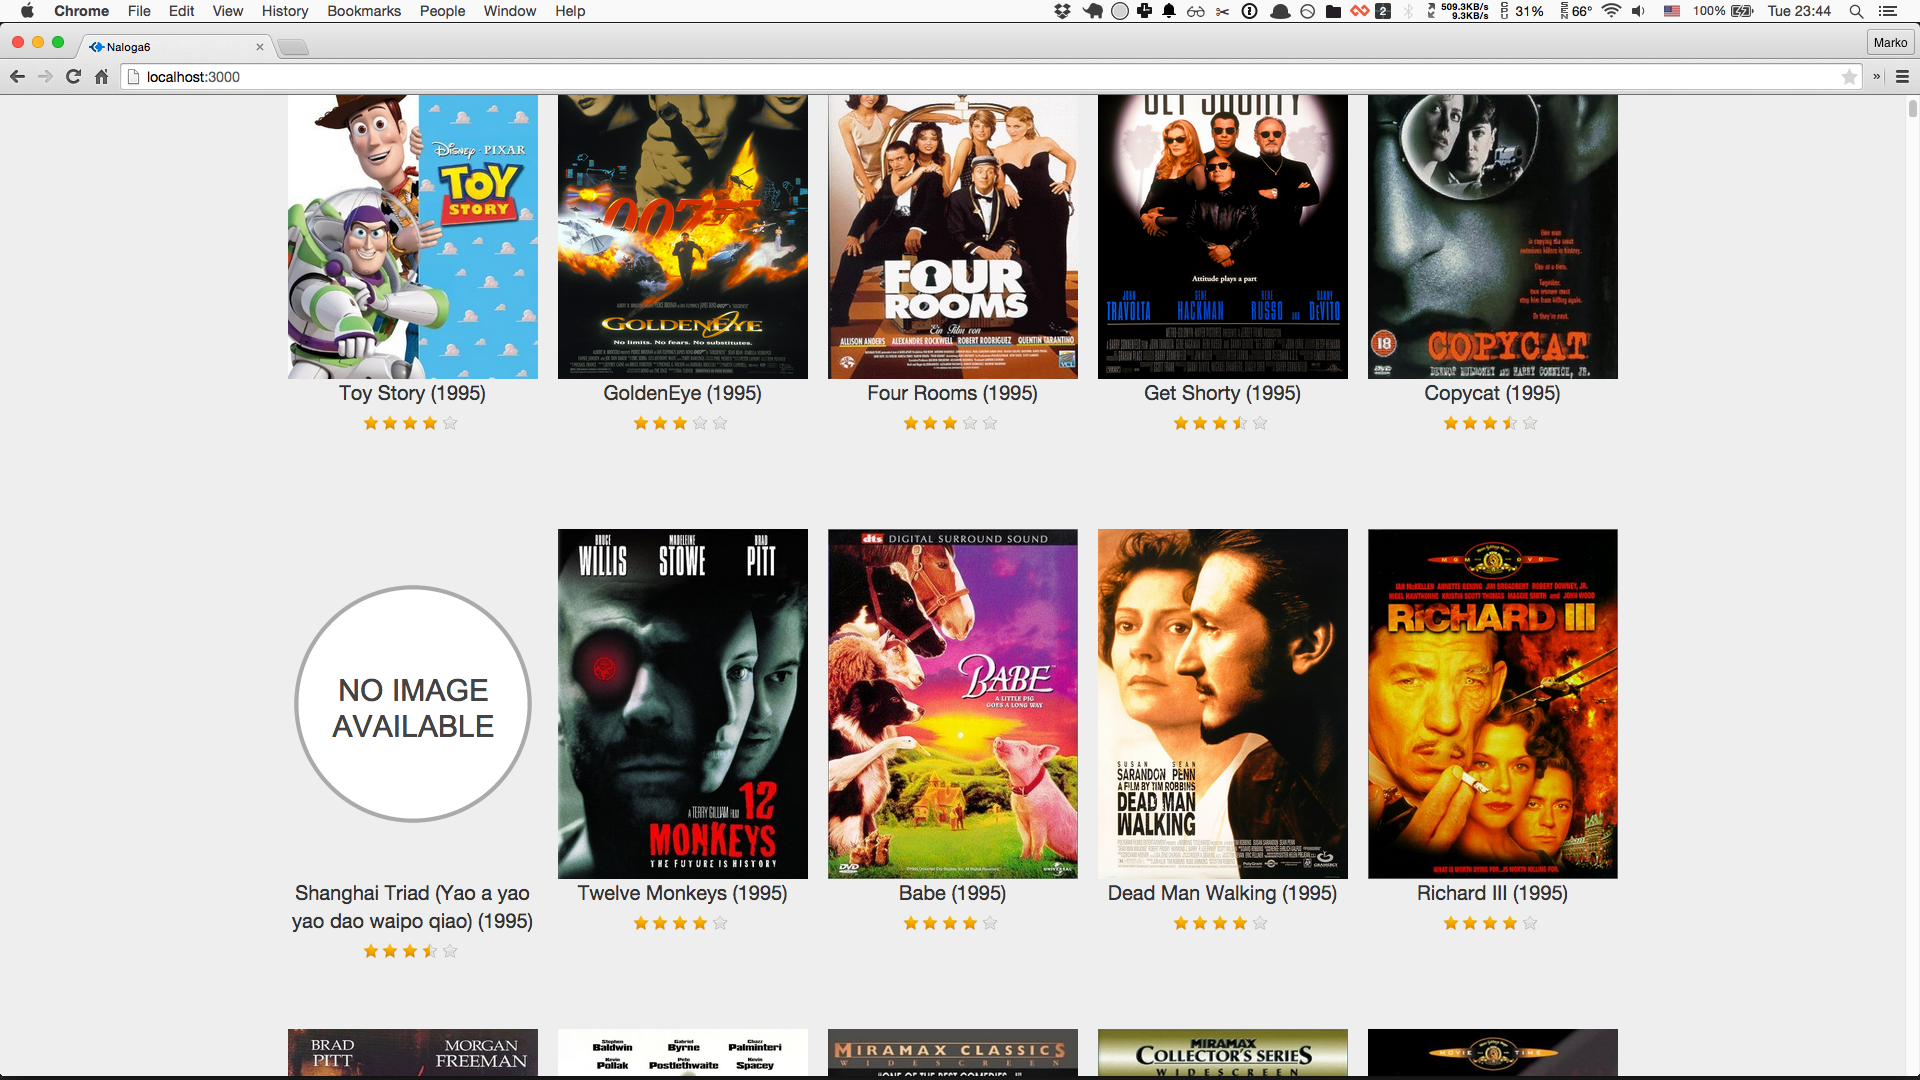
\includegraphics[width=\textwidth,height=\textheight,keepaspectratio]{filmi-vsi.png}
\caption{Pregled vseh filmov.}
\label{slika1}
\end{center}
\end{figure}

\begin{figure}[htbp]
\begin{center}
  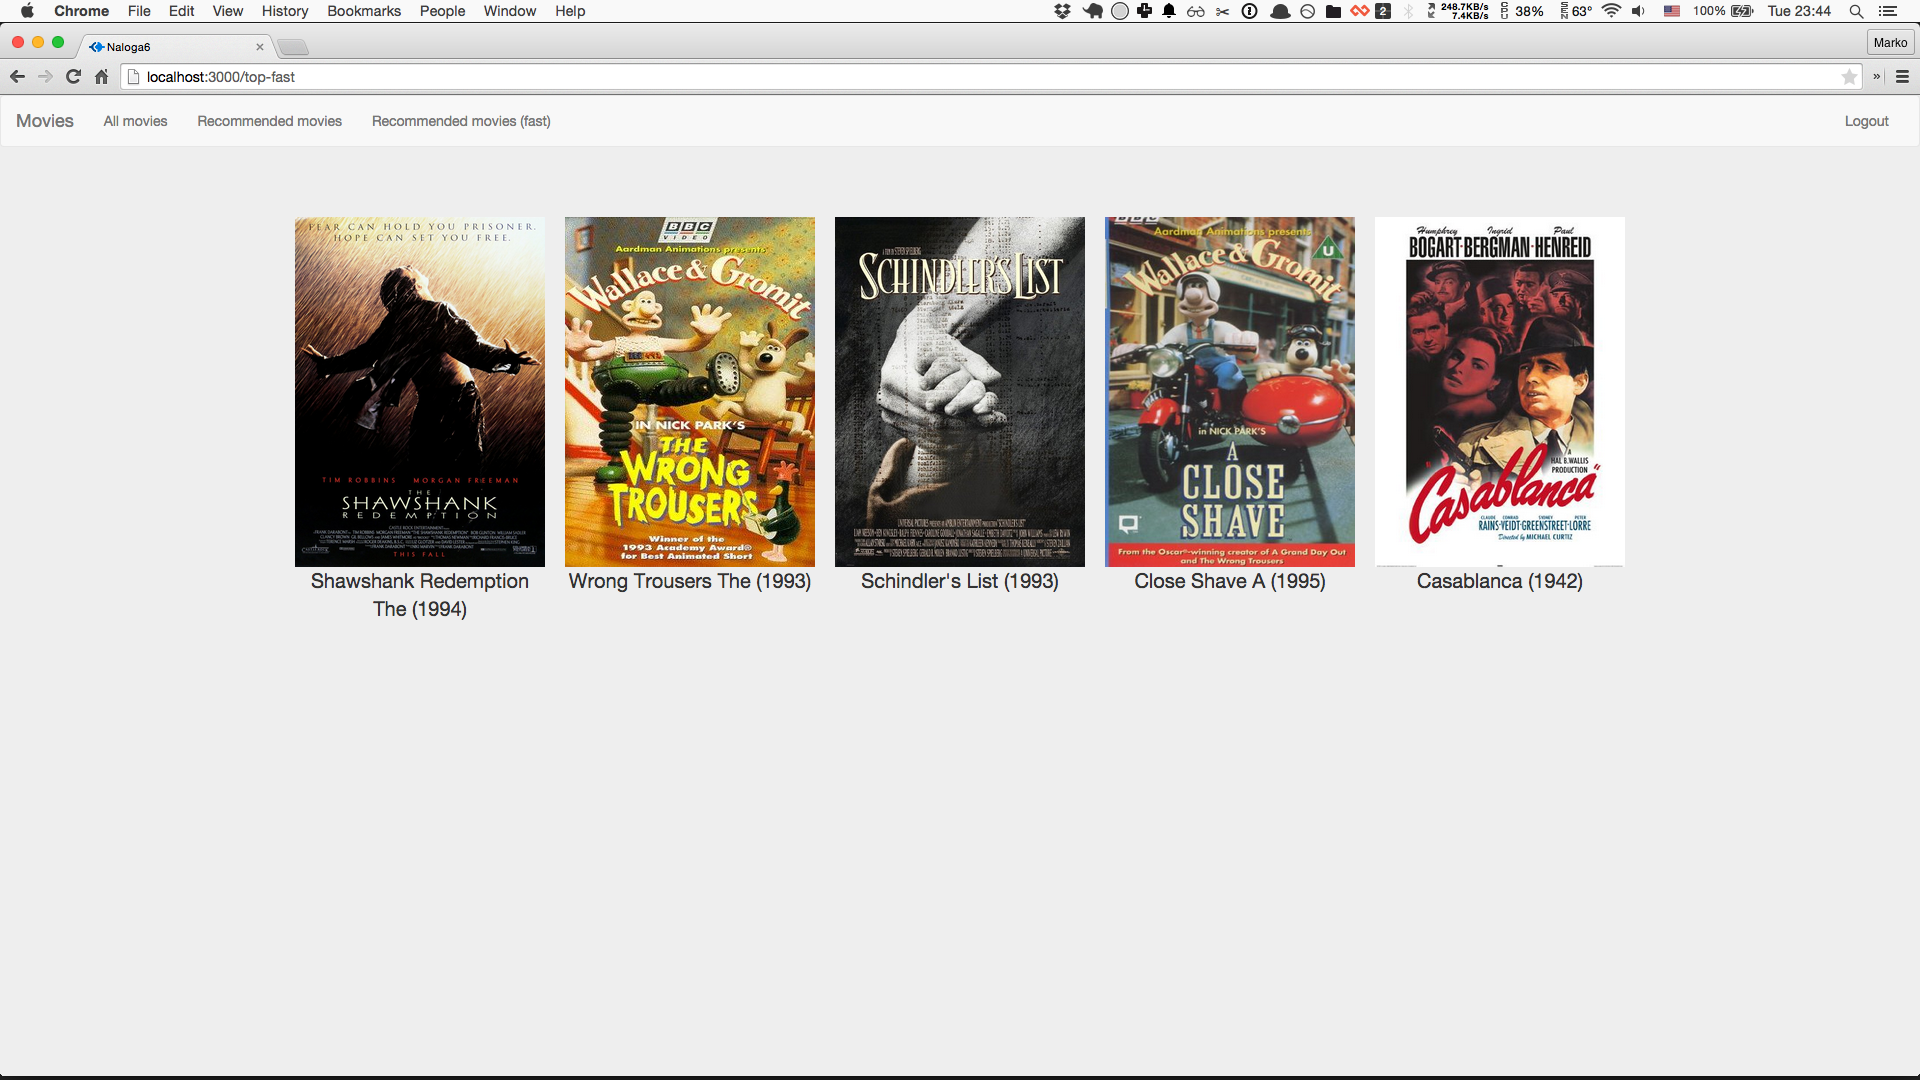
\includegraphics[width=\textwidth,height=\textheight,keepaspectratio]{filmi-top.png}
\caption{Pregled proporočenih filmov.}
\label{slika2}
\end{center}
\end{figure}


\section{Izjava o izdelavi domače naloge}
Domačo nalogo in pripadajoče programe sem izdelal sam.

\end{document}
